

\tikzset{every picture/.style={line width=0.75pt}} %set default line width to 0.75pt        

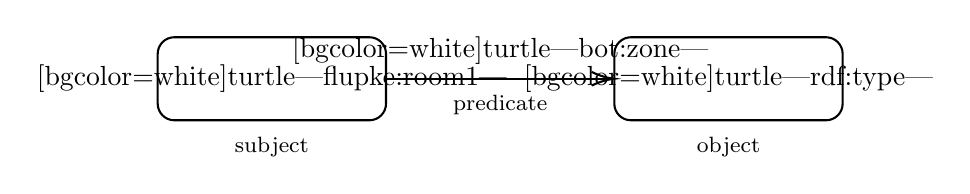
\begin{tikzpicture}[x=0.75pt,y=0.75pt,yscale=-1,xscale=1]
    %uncomment if require: \path (0,300); %set diagram left start at 0, and has height of 300

    %Rounded Rect [id:dp16428191799546488] 
    \draw   (80,68) .. controls (80,63.58) and (83.58,60) .. (88,60) -- (182,60) .. controls (186.42,60) and (190,63.58) .. (190,68) -- (190,92) .. controls (190,96.42) and (186.42,100) .. (182,100) -- (88,100) .. controls (83.58,100) and (80,96.42) .. (80,92) -- cycle ;
    %Rounded Rect [id:dp211253547738401] 
    \draw   (300,68) .. controls (300,63.58) and (303.58,60) .. (308,60) -- (402,60) .. controls (406.42,60) and (410,63.58) .. (410,68) -- (410,92) .. controls (410,96.42) and (406.42,100) .. (402,100) -- (308,100) .. controls (303.58,100) and (300,96.42) .. (300,92) -- cycle ;
    %Straight Lines [id:da3976910390317223] 
    \draw    (190,80) -- (298,80) ;
    \draw [shift={(300,80)}, rotate = 180] [color={rgb, 255:red, 0; green, 0; blue, 0 }  ][line width=0.75]    (10.93,-3.29) .. controls (6.95,-1.4) and (3.31,-0.3) .. (0,0) .. controls (3.31,0.3) and (6.95,1.4) .. (10.93,3.29)   ;

    % Text Node
    \draw (135,80) node   [align=left] {\mintinline[bgcolor=white]{turtle}|flupke:room1|};
    % Text Node
    \draw (355,80) node   [align=left] {\mintinline[bgcolor=white]{turtle}|rdf:type|};
    % Text Node
    \draw (245,66.5) node   [align=left] {\mintinline[bgcolor=white]{turtle}|bot:zone|};
    % Text Node
    \draw (135,113) node  [font=\footnotesize] [align=left] {subject};
    % Text Node
    \draw (355,113) node  [font=\footnotesize] [align=left] {object};
    % Text Node
    \draw (245,92.5) node  [font=\footnotesize] [align=left] {predicate};


\end{tikzpicture}
